\newpage
\section{Билет 18. Линейно упругое тело. Модуль Юнга, коэффициент Пуассона, коэффициненты Ламе. Связь этих коэффициентов между собой. Их физический смысл. Уравнения Ламе.}

\begin{center}
	\textit{\underline{Линейно упругое тело}}
\end{center}
\quad[Э-137]Среда называется \textbf{линейно-упругой}, или подчиняется закону Гука, если при постоянной температуре компоненты тензора напряжений являются линейными функциями компонент тензора деформации.

\quad Если в качестве начального (недеформированного) состояния выбрано состояние, в котором отсутствуют напряжения, т.е. $p^{ij}=0$ при $\epsilon_{ij}=0$, то эти линейные функции имеют вид: $$p^{ij}=A^{ijkl}\epsilon_{kl},$$
Коэффициенты $A^{ijkl}$ называются модулями упругости или упругими коэффициентами.

\begin{center}
	\textit{\underline{Закон Гука, модуль Юнга, коэф-ты Пуассона, Ламе, их связь}}
\end{center}


\quad Обобщённый закон Гука при произвольном деформировании при постоянной температуре для анизотропной среды: $$p^{ij}=A^{ijkl}\epsilon_{kl},$$
\quad Закон Гука для изотропной среды при изотермическом деформироваиии: $$p^{ij} = \lambda I_1(\epsilon)\delta^{ij}+2\mu \epsilon^{ij},$$
$I_1(\epsilon)$ - первый инвариант тензора деформаций, $\lambda, \mu$ - \textbf{коэффициенты Ламе}.

Из закона Гука имеем:
$$ \begin{cases}
p^{11} = \lambda I_1(\epsilon) + 2 \mu \epsilon_{11}\\
p^{22} = \lambda I_1(\epsilon) + 2 \mu \epsilon_{22}\\
p^{33} = \lambda I_1(\epsilon) + 2 \mu \epsilon_{33}
\end{cases},$$
Суммируем три вышенаписанных уравнения, получаем: $$I_1(p) = (3\lambda + 2\mu)I_1(\epsilon)  $$
Подставляем вместо $I_1(\epsilon)$, выражаем $\epsilon^{ij}$: $$\epsilon^{ij} = \frac{p^{ij}}{2\mu} - \frac{\lambda}{2\mu (3\lambda + 2\mu)}I_1(p)$$
Введём следующие обозначения: $$\frac{1}{2\mu} = \frac{1+\sigma}{E}, \qquad \frac{\lambda}{2\mu (3\lambda + 2\mu)}=\frac{\sigma}{E}$$
Выразим их через кожффициенты Ламэ (\textbf{связь коэффициентов}): $$E = \frac{\mu(3\lambda + 2\mu)}{\lambda + \mu}, \qquad \sigma = \frac{\lambda}{2(\lambda + \mu)}$$
E называется \textbf{модулем Юнга}, $\sigma$ - \textbf{коэффициентом Пуассона}.


\begin{center}
	\textit{\underline{Физический смысл коэффициентов}}
\end{center}
\begin{wrapfigure}{L}{0.5\textwidth}
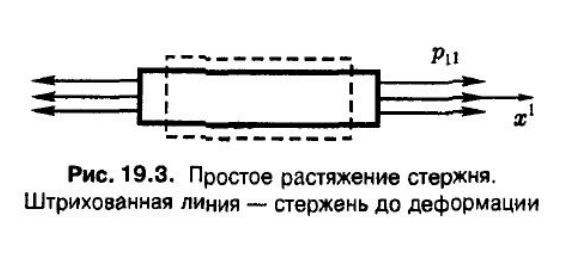
\includegraphics[width=0.5\textwidth]{18/pic1.JPG}
\caption{1}
\label{ris:image1}
\end{wrapfigure}
\quad Рассмотрим простое растяжение стержня вдоль оси $x^1$ (-> \ref{ris:image1} <-), т.е. состояние, в котором $p^{11}\neq0$, а все остальные $p^{ij}=0$. Закон Гука для простого растяжения стержня имеет вид: $$\frac{F}{S} \sim \frac{\triangle l}{l_0} ,$$
F - растягивающая сила, S - площадь поперечного сечения стержня, $\triangle l$ - удлинение стержня, $l_0$ - начальная длина стержня. $\frac{F}{S} = p_{xx}$ (если ось х направлена по силе), а $\frac{\triangle l}{l_0} = \epsilon_{xx}$ при малых деформациях. Из формул выше получаем: $$\epsilon^{11} = \frac{1}{E}p^{11}$$

Таким образом, \textbf{модуль Юнга} E - коэффициент пропорциональности между напряжением $p^{11}=\frac{F}{S}$ и относительным удлинением $\epsilon^{11}=\frac{\triangle l}{l}$ при простом растяжении стержня.
\begin{wrapfigure}{R}{0.3\textwidth}
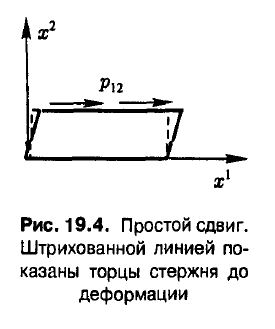
\includegraphics[width=0.3\textwidth]{18/pic2.JPG}
\caption{\label{ris:image2}2}
\end{wrapfigure}
Далее, из тех же формул, получаем, что при простом растяжении вдоль оси $x^1$ $$\epsilon^{22} = -\frac{\sigma}{E}p^{11}=-\sigma \epsilon^{11}$$
Обычно при растяжении стержень становится тоньше, т.е. $\epsilon^{22} < 0$ при $\epsilon^{11} > 0$. Таким образом, \textbf{коэффициент Пуассона} $\sigma$ - коэффициент пропорциональности между относительным сжатием в поперечном направлении и относительным удлинением в продольном направлении при простом растяжении стержня.

\quad Рассмотрим простой сдвиг (-> \ref{ris:image2} <-), т.е. состояние, в котором в декартовой системе координат $p^{12}\neq 0, \quad p^{21}=p^{12}$, а остальные компоненты $p^{ij}=0$. Тогда из закона Гука получаем: $$\epsilon^{12} = \frac{1+\sigma}{E}p^{12} = \frac{p^{12}}{2\mu}, \quad p^{12} = 2\mu \epsilon^{12}$$
В случае малых деформаций $$\epsilon^{12} = \frac{1}{2}\chi^{12},$$
где $\chi^{12}$ - изменение угла между волокнами, лежавшими до деформации вдоль осей $x^1$, $x^2$. Следовательно, коэффициент $\mu$ - это коэффициент пропорциональности между сдвигающими напряжением и изменением угла между соответствующими волокнами при простом сдвиге. Поэтому $\mu$ называют \textbf{модулем сдвига}. 

\begin{center}
	\textit{\underline{Уравнения Ламе}}
\end{center}
\quad Схема получения уравнений Ламе (Навье-Ламе) такова:
\begin{itemize}
\item В уравнениях движения выражаем $p^{ik}$ с помощью закона Гука через $\epsilon^{ik}$;

Уравнение движения в общем виде: $$\rho\frac{d\vec{v}}{dt} = \rho \vec{F} + \frac{\partial (p^{ij}\vec{e}_i)}{\partial x_j}$$
В случае, когда перемещения тела малы, выражение для левой части можно упростить: $$\vec{v} = \frac{d \vec{w}}{dt}, v^i = \frac{d w^i}{dt} = \frac{\partial w^i}{\partial t} + v^k \triangledown w^i \approx \frac{\partial w^i}{\partial t},$$
где $w^i$ - компоненты вектора перемещения. Т.е. с точностью до малых высшего порядка: $$\frac{d v^i}{dt} = \frac{\partial^2 w^i}{dt^2}$$
Уравнение движения в линейной теории упругости: $$\rho_0\frac{\partial^2 w^i}{\partial t^2} = \rho_0 F^i + \triangledown_k p^{ik}$$
\item Подставляем $\epsilon^{ik}$ через $\triangledown^i v^k$ ($\epsilon^{ik} = \frac{1}{2}(\triangledown^i w^k + \triangledown^k w^i)$).
\end{itemize}

\textbf{Уравнения Ламе в векторной форме:} $$\rho_0\frac{\partial^2 \vec{w}}{\partial t^2} = \rho_0\vec{F} + (\lambda + \mu)grad(div\vec{w}) + \mu \triangle \vec{w}$$

\begin{center}
	\textit{\underline{additional stuff}}
\end{center}
\begin{addition}
Тензором напряжений называется тензор с компонентами $p^{ik}$, для которого выполняются соотношения $P^i_n = p^{ik}n_k$в любой системе координат, причём $P^i_n$ - компоненты вектора напряжений на площадке, компоненты нормали к которой суть $n_k$. $P^i = \{p^{i1},p^{i2},p^{i3}\}$ [Э-110]
\end{addition}
\begin{addition}
О тензорах деформаций [Э-52]
\end{addition}
